\chapter{Zásuvný modul}
\label{4-plugin}

Čtvrtá kapitola popisuje vývoj zásuvného modulu a~rozebírá důležité části kódu. 


\section{Obsah CSV}
\label{obsah}

Vstupní soubor s~měřenými daty musí být tzv.~\zk{CSV}~(\textit{comma-separated values} - hodnoty oddělené
čárkami) soubor. Oddělování čárkami představuje pro čtení souboru zásuvným modulem zásadní podmínku.
Software v~měření radioaktivity (a~mnohdy i~jiných atributů) běžně používaný k~zápisu obvykle
produkuje právě soubory s~koncovkou~.\zk{CSV} a~s~nezbytnými i~doplňujícími atributy. Na pořadí
atributů nezáleží. 

Povinné části a~jejich označení v~hlavičce souboru: 
\begin{itemize}

	\item RECS: Pod označením RECS se skrývá číslo bodu. Tato položka je nezbytná pouze
	v~případě \textit{posunu o~hodnoty} (kvůli přepisu označení bodu z~důvodu zachování úzu číslování
	od čísla~0). Avšak číslování bodů zajišťuje čitelnost dat, pročež je silně doporučováno vždy. 
	
	\item Lat\_deg: Lat\_deg označuje sloupec obsahující zeměpisnou šířku snímaného bodu na elipsoidu.
	Za referenční elipsoid, na němž se úloha vypočítává, byl zvolen nejběžněji užívaný
	elipsoid~\zk{WGS84}. 
	
	\item Lon\_deg: Lon\_deg označuje sloupec obsahující zeměpisnou délku snímaného bodu na elipsoidu.
	Za referenční elipsoid, na němž se úloha vypočítává, byl zvolen nejběžněji užívaný
	elipsoid~\zk{WGS84}. 
	
	\item mereni: mereni obsahuje měřenou hodnotu (v~prezentovaném případě hodnotu radioaktivity, ale
	sloupec by mohl obsahovat jakoukoli jinou, i~nečíselnou hodnotu). 
	
	\item Gtm\_sec: Čas měření ve vteřinách. Není důležité, jaký typ udávání času daný soubor
	podporuje (zda například počítá vteřiny od nějakého roku, nebo od začátku měření), počítá
	se s~rozestupy mezi jednotlivými údaji. 

\end{itemize}

Soubor bývá doplněn o~data pro zásuvný modul zbytná, například číslo linie, souřadnice na jiném
referenčním tělese, nadmořskou výšku, jiný systém času nebo datace. 

  \begin{figure}[H]
   \centering
	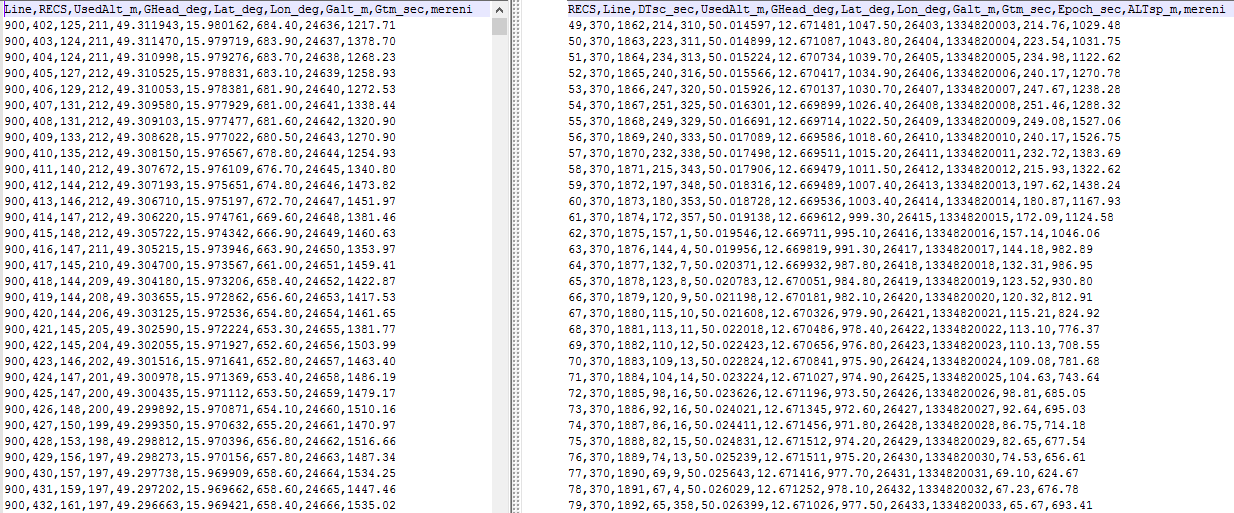
\includegraphics[scale=0.5]{./pictures/ukazka-vstup.png}
	\caption[Ukázka dvou typů vstupních souborů]{Ukázka dvou typů vstupních souborů
      \label{fig:ukazka-vstup}}
  \end{figure}

\section{Tělo zásuvného modulu}
\label{telo}

\section{Posun o hodnoty}
\label{by_points}

\section{Posun o konstantní vzdálenost}
\label{by_distance}

\subsection{Výpočet azimutu}
\label{azimut}

\subsection{První geodetická úloha}
\label{prvniguplugin}

\section{Posun o konstantní čas (proměnnou vzdálenost)}
\label{by_seconds}

\section{Licence}
\label{licence}



